\documentclass[10pt, a4paper]{article}

%%% SST LAB PROTOCOLL PREAMBLE
%%% 2019
%%%%%%%%%%%%%%%%%%%%%%%%%%%%%%%


%%% PACKAGES
%%%%%%%%%%%%%%%%%%%%%%%%%%%

\usepackage[ngerman]{babel}

\usepackage[utf8]{inputenc}
\usepackage{amsmath}
\usepackage{pgfplots}
\usepackage{tikz}
\usepackage[many]{tcolorbox}
\usepackage{graphicx}
\graphicspath{ {./graphics/} }
\usepackage{pdfpages}
\usepackage{dashrule}
\usepackage{float}
\usepackage{siunitx}
\usepackage{trfsigns}
\usepackage{booktabs}
\usepackage[european]{circuitikz}
\usepackage{tcolorbox}

%%% DOCUMENT GEOMETRY
%%%%%%%%%%%%%%%%%%%%%%%%%%%

\usepackage{geometry}
\geometry{
 a4paper,
 total={0.6180339887498948\paperwidth,0.6180339887498948\paperheight},
 top = 0.1458980337503154\paperheight,
 bottom = 0.1458980337503154\paperheight
 }
\setlength{\jot}{0.013155617496424828\paperheight}
\linespread{1.1458980337503154}

\setlength{\parskip}{0.013155617496424828\paperheight} % paragraph spacing


%%% COLORS
%%%%%%%%%%%%%%%%%%%%%%%%%%%

\definecolor{red1}{HTML}{f38181}
\definecolor{yellow1}{HTML}{fce38a}
\definecolor{green1}{HTML}{95e1d3}
\definecolor{blue1}{HTML}{66bfbf}
\definecolor{hsblue}{HTML}{00b1db}
\definecolor{hsgrey}{HTML}{afafaf}

%%% CONSTANTS
%%%%%%%%%%%%%%%%%%%%%%%%%%%
\newlength{\smallvert}
\setlength{\smallvert}{0.0131556\paperheight}


%%% COMMANDS
%%%%%%%%%%%%%%%%%%%%%%%%%%%

% differential d
\newcommand*\dif{\mathop{}\!\mathrm{d}}

% horizontal line
\newcommand{\holine}[1]{
  	\begin{center}
	  	\noindent{\color{hsgrey}\hdashrule[0ex]{#1}{1pt}{3mm}}\\%[0.0131556\paperheight]
  	\end{center}
}

% mini section
\newcommand{\minisec}[1]{ \noindent\underline{\textit {#1} } \\}

% quick function plot
\newcommand{\plotfun}[3]{
  \vspace{0.021286\paperheight}
  \begin{center}
    \begin{tikzpicture}
      \begin{axis}[
        axis x line=center,
        axis y line=center,
        ]
        \addplot[draw=red1][domain=#2:#3]{#1};
      \end{axis}
    \end{tikzpicture}
  \end{center}
}

% box for notes
\newcommand{\notebox}[1]{

\tcbset{colback=white,colframe=green1!100!black,title=Note!,width=0.618\paperwidth,arc=0pt}

 \begin{center}
  \begin{tcolorbox}[]
   #1 
  \end{tcolorbox}
 
 \end{center} 
 
}

% box for equation
\newcommand{\eqbox}[2]{
	
	\tcbset{colback=white,colframe=green1!100!black,title=,width=#2,arc=0pt}
	
	\begin{center}
		\begin{tcolorbox}[ams align*]
				#1
		\end{tcolorbox}
		
	\end{center} 
	
}
% END OF PREAMBLE
\usepackage{todonotes}

\newcommand{\upperRomannumeral}[1]{\uppercase\expandafter{\romannumeral#1}}
\newtcbox{\inlinecodee}{on line, boxrule=0pt, boxsep=0pt, top=2pt, left=2pt, bottom=2pt, right=2pt, colback=gray-2, colframe=white, fontupper={\ttfamily \footnotesize}}


\begin{document}

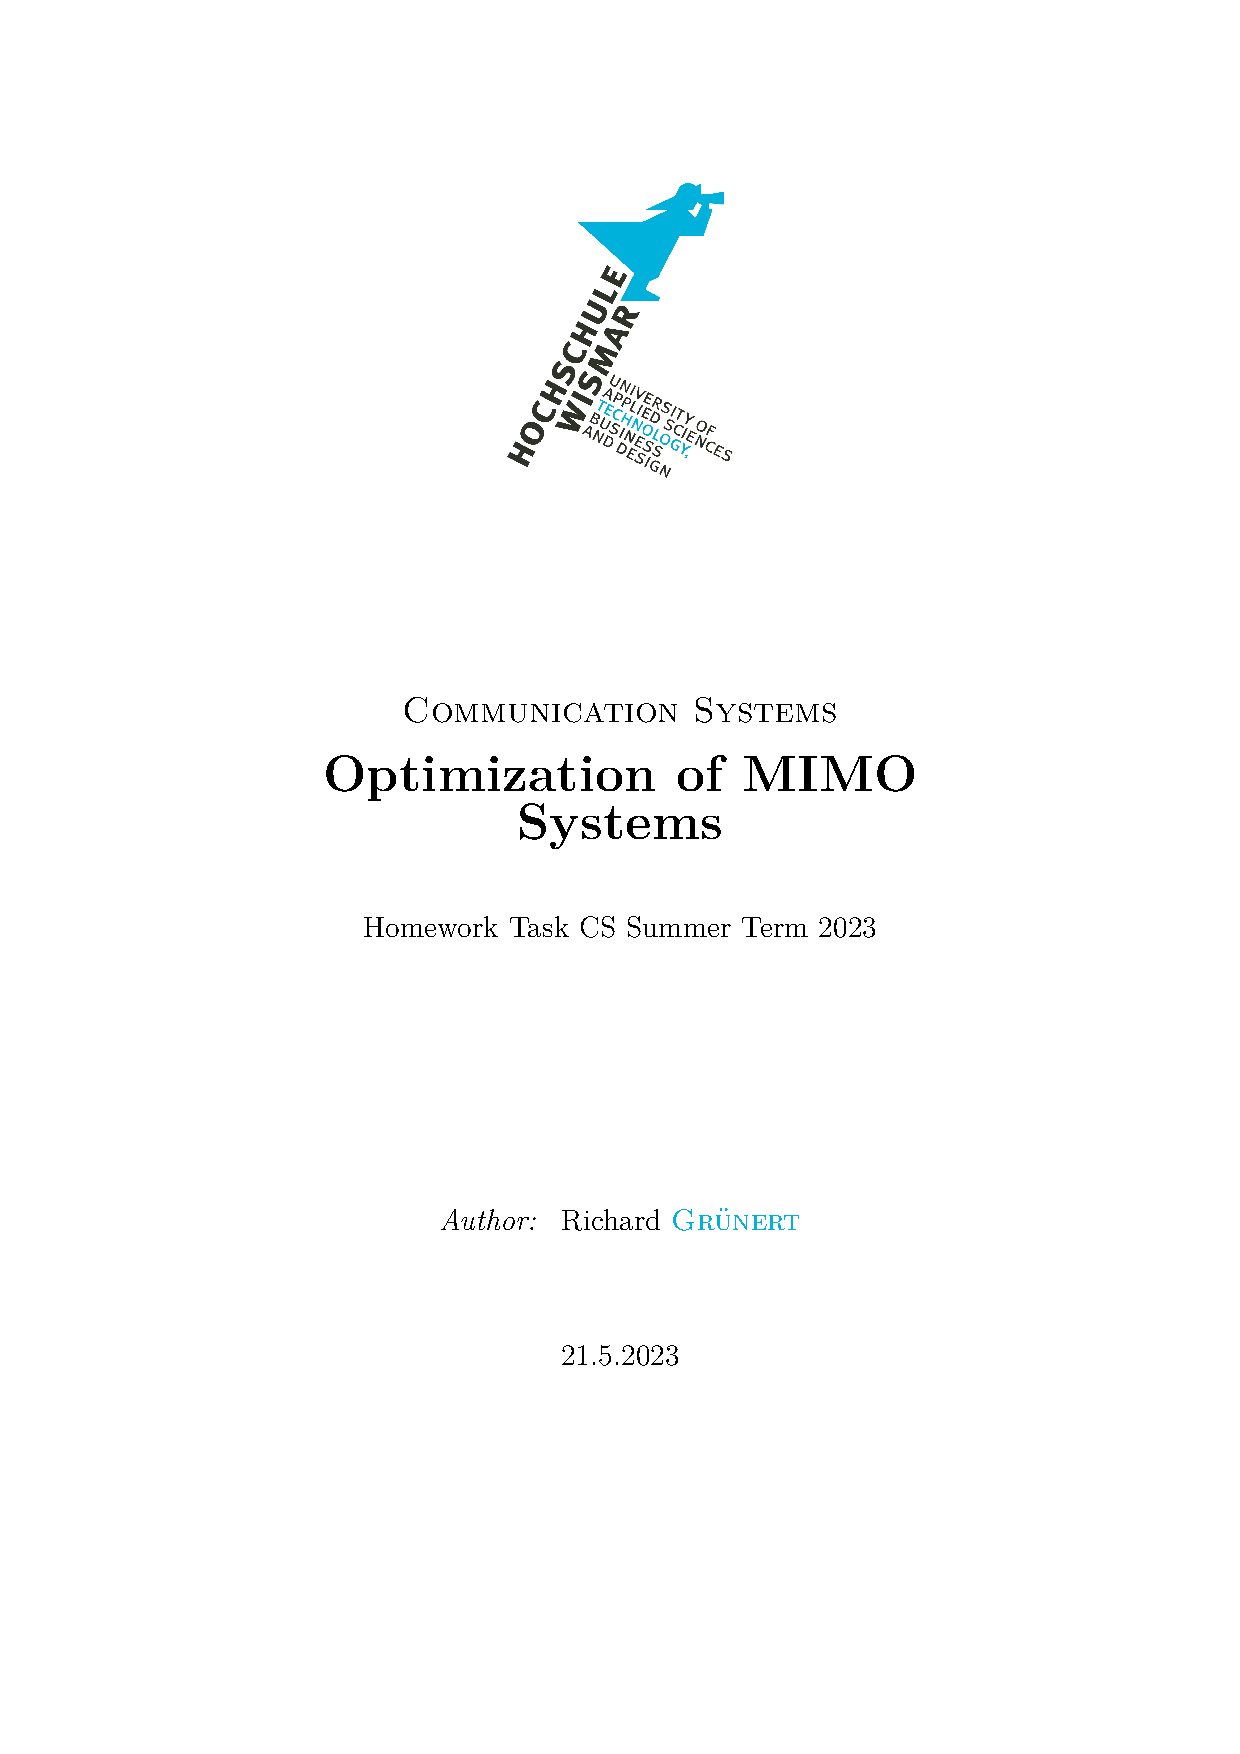
\includepdf{./titlepage/titlepage.pdf}

\section{Procedure / Method}
Using \textsc{Matlab Simulink}\texttrademark{}, the provided model file \inlinecodee{M12\_MIMO\_flexBitLoad.slx} as well as the \inlinecodee{initial\_.m} file have been extended to solve the given tasks. Figure \ref{fig:system_screenshot} shows a screenshot of the model in Simulink.\\

\begin{figure}[H]
\centering
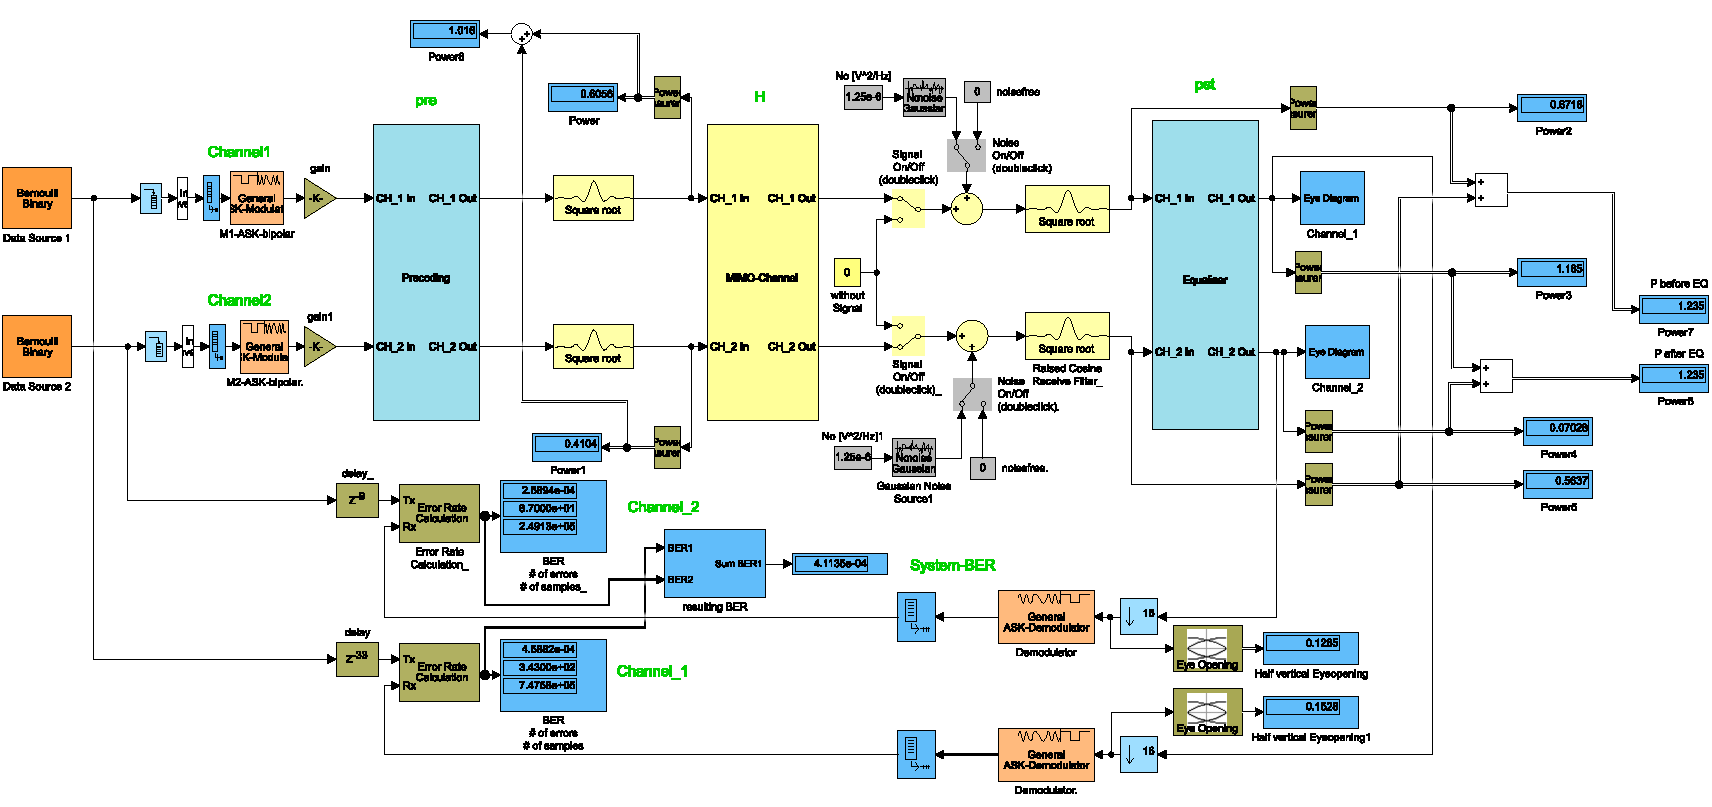
\includegraphics[width=0.764\textwidth]{graphics/mimo_model.pdf}
\caption{2x2 MIMO Simulation System}\label{fig:system_screenshot}
\end{figure}

The goal is to send a total of $4\,\si{\bit}$ per time step with an allowed total transmit power of $1\,\si{\volt\squared}$ while minimizing the BER. This can be done with different bitloads, i.e. different constellations for each layer as well as different power allocations.

\section{Model Check}
A detection SNR of $19\,\si{\deci\bel}$ was required. As a linear ratio, this equals approximately $79.43$.
Since the transmit power is $1\,\si{\volt\squared}$, the noise power should be $\frac{1\,\si{\volt\squared}}{79.43}=0.01256\,\si{\volt\squared}$. In the model, the summed noise power of each MIMO receiver (simulation without transmit sigal) is $0.01238\,\si{\volt\squared}$ which shows that it is set up correctly.


\section{Raw Transmission}
When transmitting without any added noise and additional signal processing, one finds that the original 4-ASK now results in 16 different symbol amplitudes after passing through the channel (see figure \ref{figure:raw1}). The resulting BER is $0.1$ with channel 1 having basically no errors.

\begin{figure}[h]
\centering
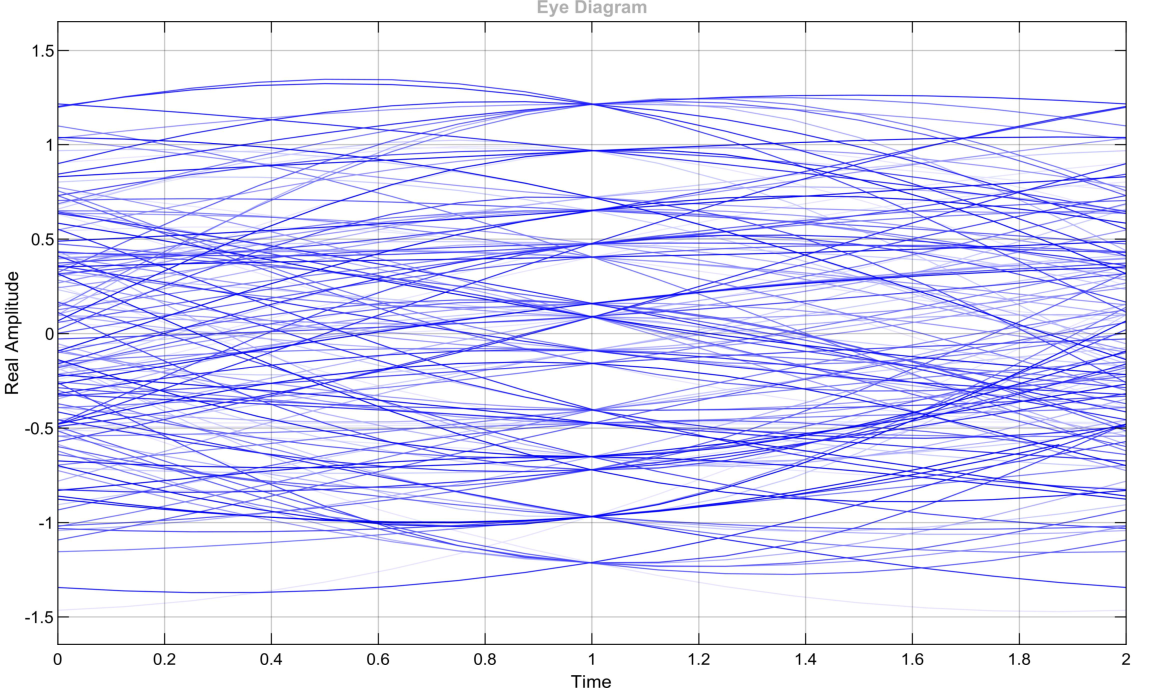
\includegraphics[width=0.618\textwidth]{graphics/mimo_eye_raw_ch_1.pdf}
\caption{Eye at receiver side of channel 1 without any measures.}\label{figure:raw1}
\end{figure}


With the addition of noise, the BER becomes $0.088$. This is lower than without noise in this case because in the simulation without noise no errors occured which scewed the BER result.



\section{Zero-Forcing Equalization}
Zero-Forcing equalization is easy to implement for this particular model since the channel matrix $H$ is a regular matrix for which an inverse exists. This inverse is
\[H^{-1} = \left[\begin{matrix}
                   1.1013 & -0.2599\\
                   -0.4826 & 1.2375\\
\end{matrix}\right]\]

This has to be multiplied by the incoming signal. However, this approach is also expected to increase the noise power.
In the model, the inverse matrix was set as the equalization block parameter. The precoding stayed the same (no influence). The result is an equal eye opening of $0.314\,\si{\volt}$ on both channels (see figure \ref{fig:zf1}) which closely matches the $U_{s}$ but the noise power after the equalizer is now approximately $0.0183\,\si{\volt\squared}$ which is an increase by a factor of $1.46$. This has a negative impact on the minimum possible BER.\\

\begin{figure}[h]
\centering
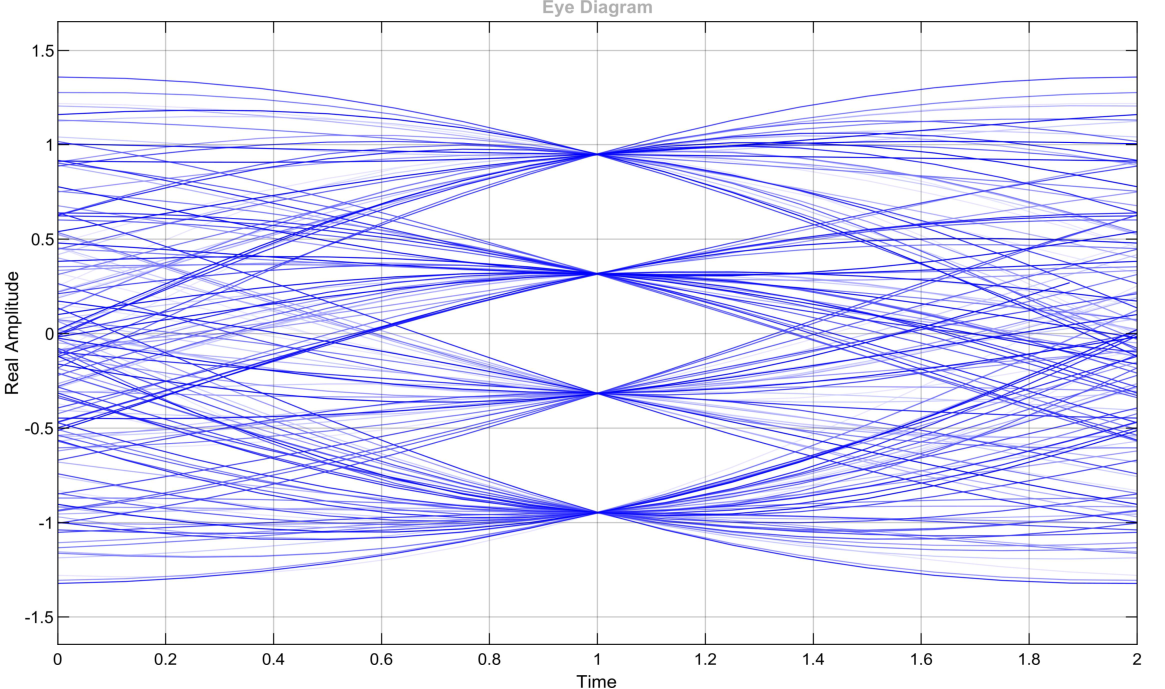
\includegraphics[width=0.618\textwidth]{graphics/mimo_eye_zeroforcing_ch_1.pdf}
\caption{Eye at receiver side of channel 1 after zero-forcing equalization.}\label{fig:zf1}
\end{figure}


The calculated and simulated BER match quite well. The slight difference in channel 1 might be because of the low absolute number of errors in channel 1 (just 41 in this case) due to the limited simulation runtime.



\section{SVD}
The SVD divides the channel matrix $H$ into three components ($U, S, V^{H}$). The inverse operations for these components are then perfomed in two steps, the precoding and postcoding / equalization.

Precoding happens with the conjugate transpose (here just transpose) of $U$, postcoding with $V$. Since $U$ and $V$ are unitary matrices, the multiplication by their complex conjugate yields the identity matrix. So the only term remaining is the diagonal matrix $S$ which holds the scaling factors for each channel.\\

After applying the SVD-operations, one can model the MIMO system with independent layers, where each layer has a weighting factor corresponding to the $S$-matrix entry.\\

Additionally, the constellation (bitloading) as well as the power (powerloading) each layer receives can be adjusted so that layers with a lower overall quality can be compensated.

\subsection{Plain SVD}
The results for the plain SVD without bit- or powerloading show that the quality of channel 1 is greatly increased in comparison to the zero-forcing method since the noise power is not increased. The eyes are however not equally open. They are weighted by the values of the $S$-matrix, as can be seen in figures \ref{fig:svd_plain1} and \ref{fig:svd_plain2}.
So one can expect a different performance from each layer. In this case, channel 2 basically dictates the BER since channel 1 is almost error-free.

\begin{figure}[h]
    \centering
    \begin{minipage}{0.45\textwidth}
        \centering
        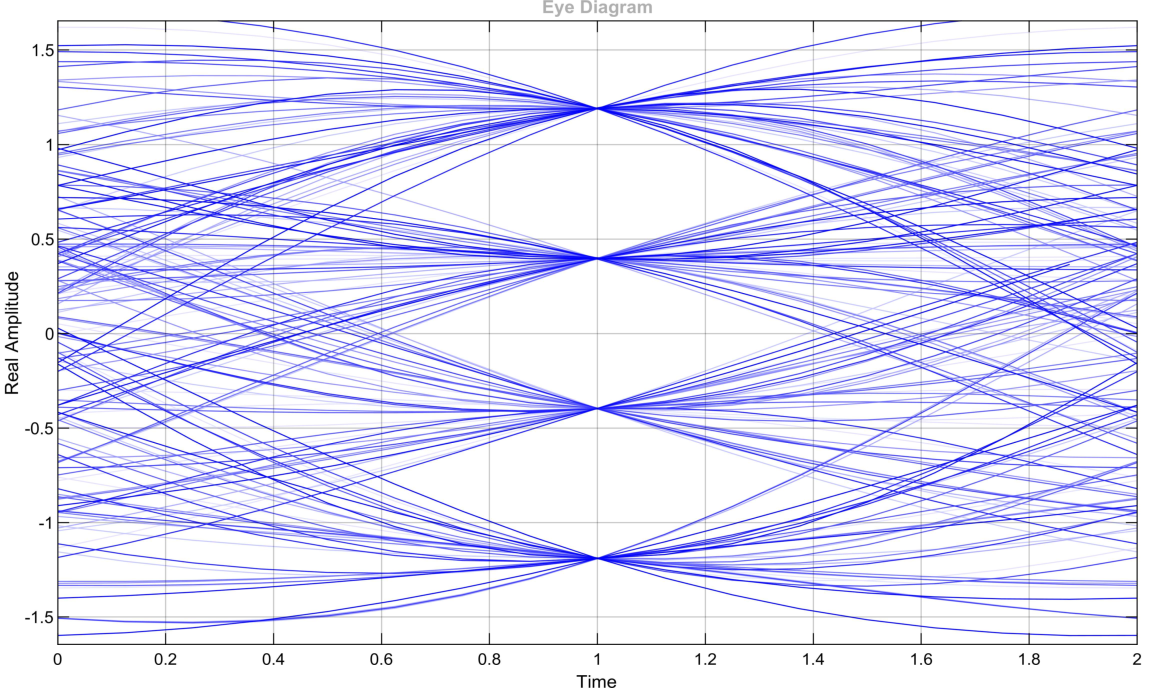
\includegraphics[width=0.764\textwidth]{graphics/mimo_eye_svd_raw_ch_1.pdf}
        \caption{Eye at receiver side of channel 1 after SVD pre- and postcoding.}\label{fig:svd_plain1}
    \end{minipage}\hfill
    \begin{minipage}{0.45\textwidth}
        \centering
        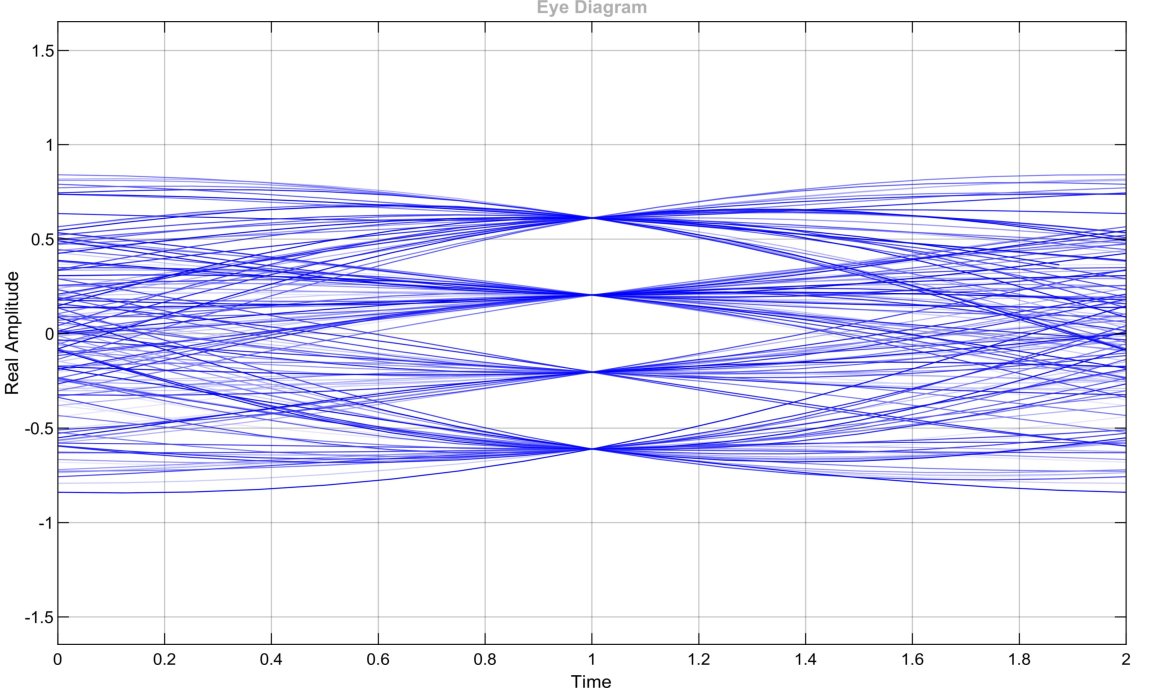
\includegraphics[width=0.764\textwidth]{graphics/mimo_eye_svd_raw_ch_2.pdf}
        \caption{Eye at receiver side of channel 2 after SVD pre- and postcoding.}\label{fig:svd_plain2}
    \end{minipage}
\end{figure}

\subsection{SVD with different Bitloads}
By chosing a different number of bits to send in each layer, a low-performing layer can receive a lower number of bits, therefore improving the total BER by simply having a lower absolute error count. However, the other layer will have to increase its number of bits per symbol if the same bitrate is desired, resulting in a reduced $U_{A}$ which increases the BER.\\

The case of $b_{l1} = 3, b_{l2}=1$ is shown in figures \ref{fig:bitload1} and \ref{fig:bitload2}. It comes quite close to the plain SVD setup but is not better.\\

\begin{figure}[h]
    \centering
    \begin{minipage}{0.45\textwidth}
        \centering
        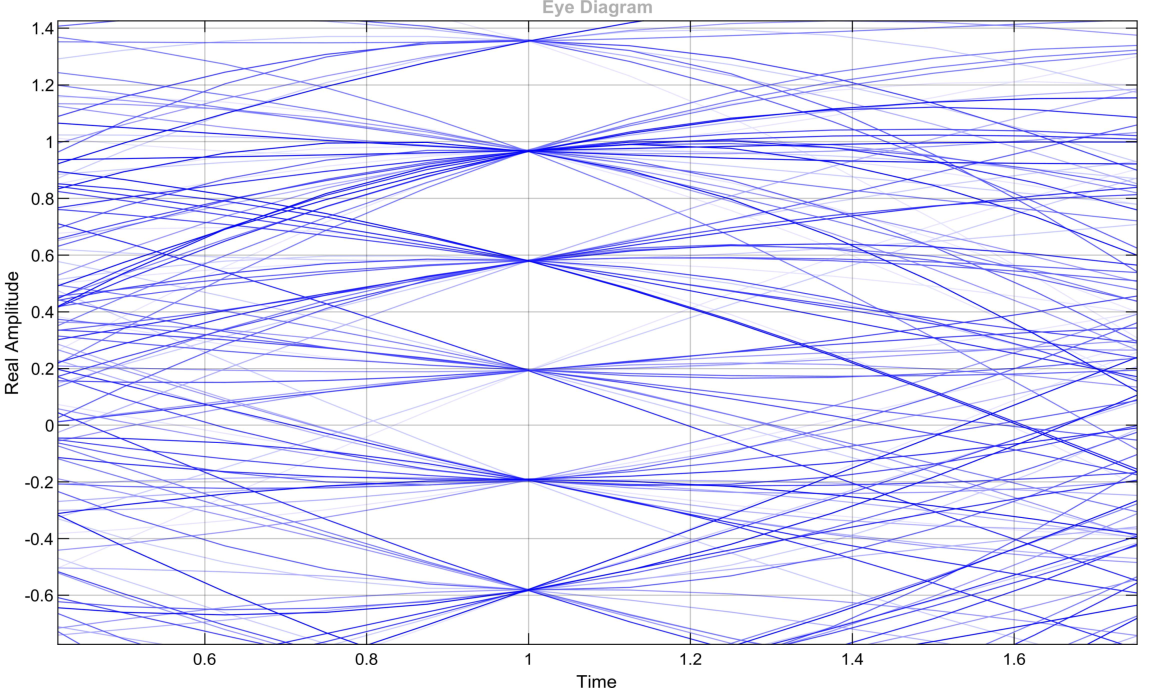
\includegraphics[width=0.764\textwidth]{graphics/mimo_eye_svd_bit82_ch_1.pdf}
        \caption{SVD receiver side of channel 1 with $s=8$}\label{fig:bitload1}
    \end{minipage}\hfill
    \begin{minipage}{0.45\textwidth}
        \centering
        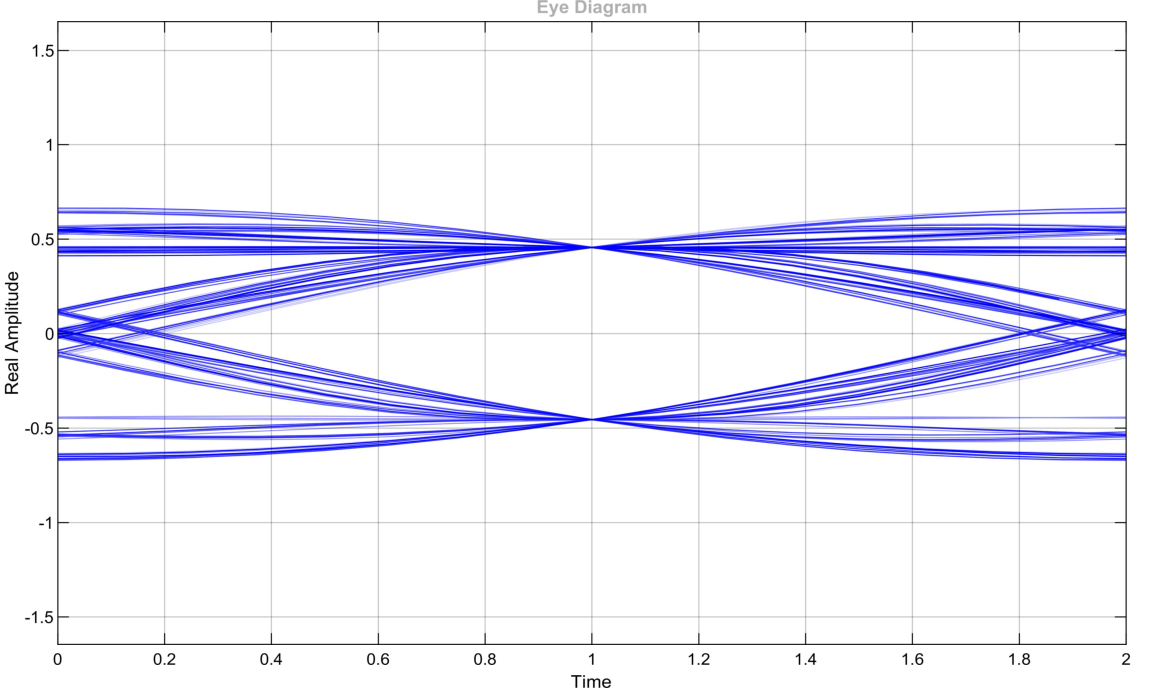
\includegraphics[width=0.764\textwidth]{graphics/mimo_eye_svd_bit82_ch_2.pdf}
        \caption{SVD receiver side of channel 2 with $s=2$}\label{fig:bitload2}
    \end{minipage}
\end{figure}


The reverse case of $b_{l1}=1, b_{l2}=3$ does not make much sense since the low-performing layer will then perform even worse due to the decreased eye and the other layer does not benefit from an increased eye.

\subsection{Optimized SVD}
The idea is to somehow make the BERs of the individual layers as equal as possible. Since this depends on the detection SNR, one can try to make the eye openings of the layers equal by employing powerloading. It only has to be guaranteed that the transmit power does not exceed $1\,\si{\volt\squared}$.\\

With this approach, the results for a bitload of $b_{l1}=2, b_{l2}=2$ are almost identical to the $b_{l1}=3, b_{l2}=1$ case and better than the zero-forcing implementation.\\

The best BER was achieved by ``trying out'', taking the equal-eye-opening case as a basis and then waiting for at least $30$ errors on each channel. The resulting factors are
\begin{align*}
  p_{l1} = 0.7091\\
  p_{l2} = 1.2236
\end{align*}

at a bitload of $b_{l1} = 2, b_{l2}=2$.

\end{document}
